% witness: 1605.07806 (`\put(2,0){\includegraphics[height=170pt]{surface-eps-converted-to}}` under `$V$`, `$P$`, `$t$`
%          labels); also 2403.09205, 1104.5392, 1509.02249, 1601.05000 (sized PDF figures rendered under-sized)
% oracle:  pdflatex 0 errors; the figure 170pt high (quadrants.pdf: 216x108 bp), the labels over it
% engines: rust INT081TR = the SVG root keeps the converter's 216x108 while the object is 469x235: ar5iv.css's
%          `width:auto;height:auto` shows the root's size, and the labels fall off the figure
% expect:  0 errors, 0 warnings; HTML (EXT=html): x1.svg's root width="469" height="235" viewBox="0 0 216 108",
%          the object width="469" height="235"
% status:  RED (INT081TR) -> GREEN (SVGSCALE)
% preload: ar5iv.sty
\documentclass{article}
\usepackage{graphicx}
\begin{document}
\begin{picture}(240,170)(2,0)
  \put(2,0){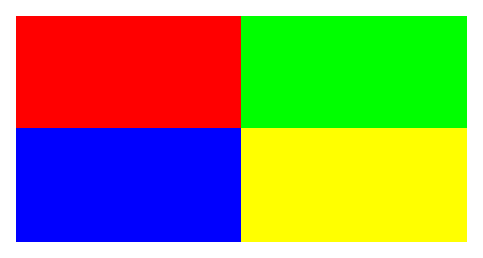
\includegraphics[height=170pt]{quadrants}}
  \put(150,150){$V$}\put(220,49){$P$}\put(50,0){$t$}
\end{picture}
\end{document}
